% Additional figures for the circuit-level SI1000 and SD6 results.
% Numbers trace to paper-rework/facts/*.csv and the run folders listed in facts/runs.csv.

\section{Additional Results}
\label{sec:additional-results}

This appendix collects the figures that support \autoref{sec:results} but are not shown there. \autoref{fig:unif2_si1000_1anc} to \autoref{fig:unif4_sd6_1anc} show uniform-interval postselection with $k = 2$, $3$ and $4$ in the one-ancilla layout, discussed in \autoref{sub:interval_results}. \autoref{fig:const0_si1000_2anc} to \autoref{fig:unif1_sd6_2anc} show terminal postselection and uniform-interval postselection with $k = 1$ for the two-ancilla layout, and \autoref{fig:threshold_grid_si1000_2anc} and \autoref{fig:threshold_grid_sd6_2anc} show its pseudo-threshold construction, all discussed in \autoref{sub:layout_comparison}. In the depth-decay figures, \autoref{fig:unif2_si1000_1anc} to \autoref{fig:unif1_sd6_2anc}, the panels follow \autoref{fig:const0_si1000_1anc} and \autoref{fig:unif1_si1000_1anc}. Each pair of panels belongs to one of $p = 10^{-4}$, $5\times10^{-4}$, $10^{-3}$, $2\times10^{-3}$, $5\times10^{-3}$ and $10^{-2}$. The left panel shows the accepted $\langle \bar{X} \rangle$ of LRB-D (blue) and $\langle Z \rangle$ of physical RB under the same noise model at the same $p$ (orange) versus depth $m$, and the right panel shows the rejected fraction. The legend of each pair sits in its right panel and labels the curves of the left panel. Where fits are drawn, they are $F(m) = A f^m$, and the legends give $\bar{F}$ per unit of depth. The two threshold-grid figures follow \autoref{fig:threshold_grid_si1000_1anc} and \autoref{fig:threshold_grid_sd6_1anc}. All $\chi^2$ values quoted below are defined as in \autoref{sub:interval_results}.

\subsection{One-Ancilla Layout, Intervals \texorpdfstring{$k = 2$}{k = 2} to \texorpdfstring{$4$}{4}}

\begin{figure}[H]
  \centering
  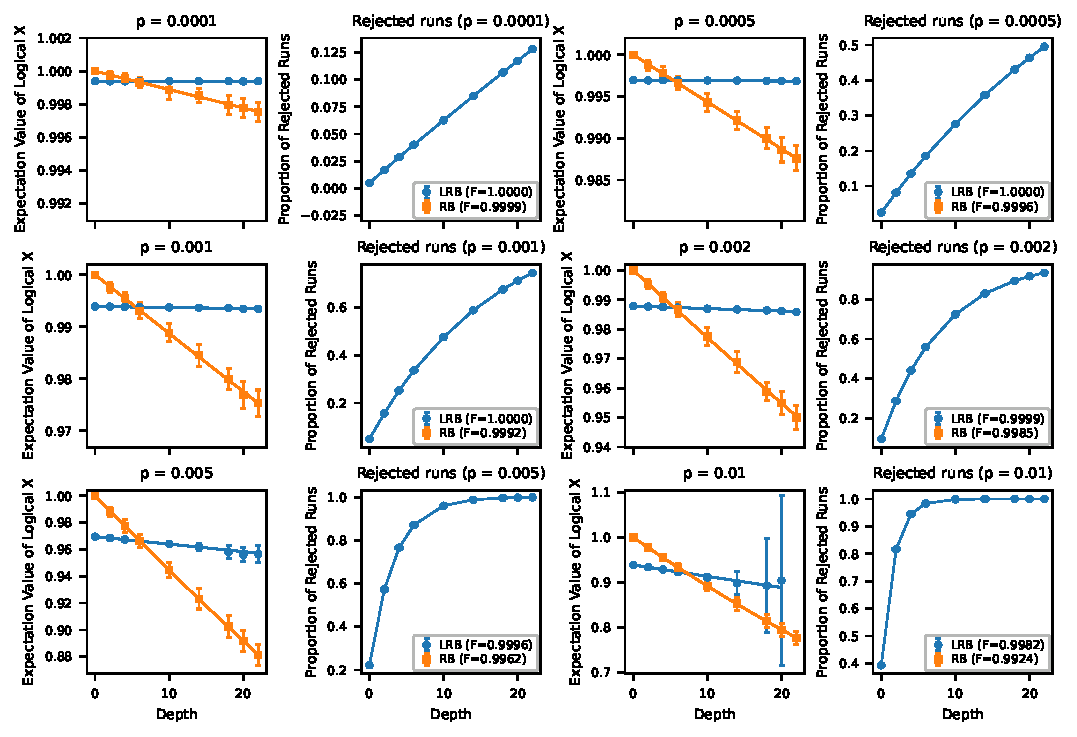
\includegraphics[width=0.78\textwidth]{figures/sdim140/si1000-1anc-unif-2-fit.pdf}
  \caption{Uniform-interval postselection with $k = 2$, one-ancilla layout, SI1000. Every depth on the grid is a multiple of 2, and the zero-offset fits stay close to the data ($\chi^2 = 0.39$ over nine depths at $p = 5\times10^{-3}$). At $p = 5\times10^{-3}$ the fitted error per unit depth is $3.9\times10^{-4}$, against $2.3\times10^{-4}$ for $k = 1$.}
  \label{fig:unif2_si1000_1anc}
\end{figure}

\begin{figure}[H]
  \centering
  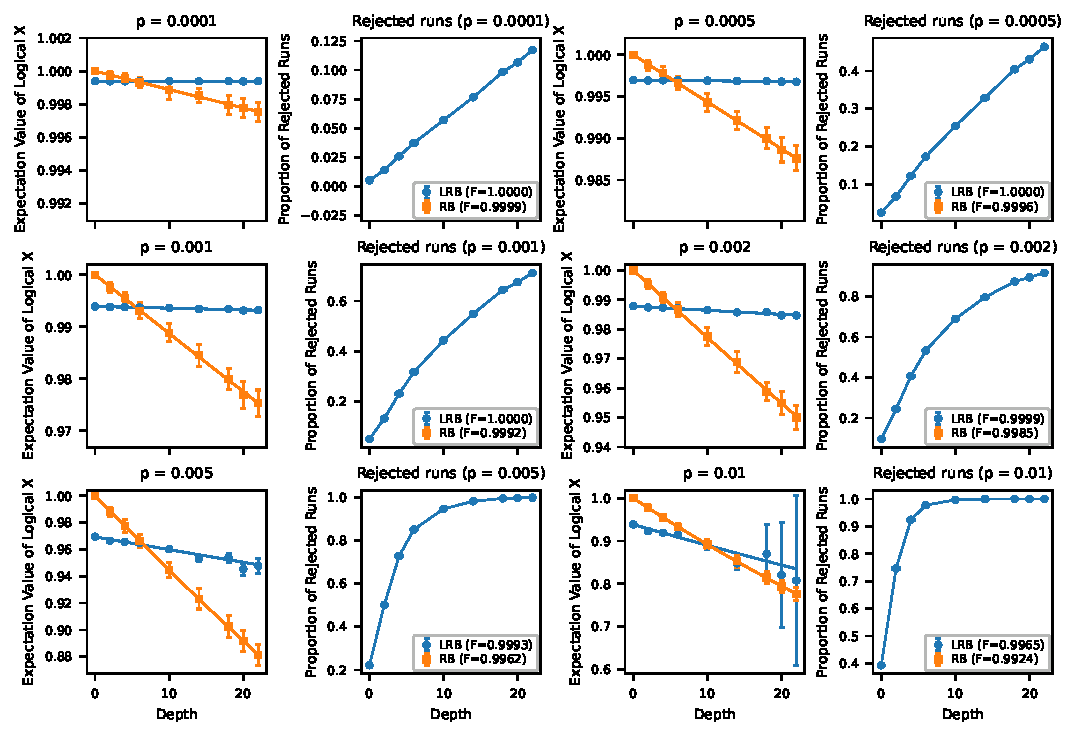
\includegraphics[width=0.78\textwidth]{figures/sdim140/si1000-1anc-unif-3-fit.pdf}
  \caption{Uniform-interval postselection with $k = 3$, one-ancilla layout, SI1000. The rejected fraction at fixed depth $m \ge 2$ is lower than for $k \le 2$, and the traces develop steps at depths that are not multiples of 3 ($\chi^2 = 12.6$ over nine depths at $p = 5\times10^{-3}$). At $p = 5\times10^{-3}$ the fitted error per unit depth is $6.6\times10^{-4}$.}
  \label{fig:unif3_si1000_1anc}
\end{figure}

\begin{figure}[H]
  \centering
  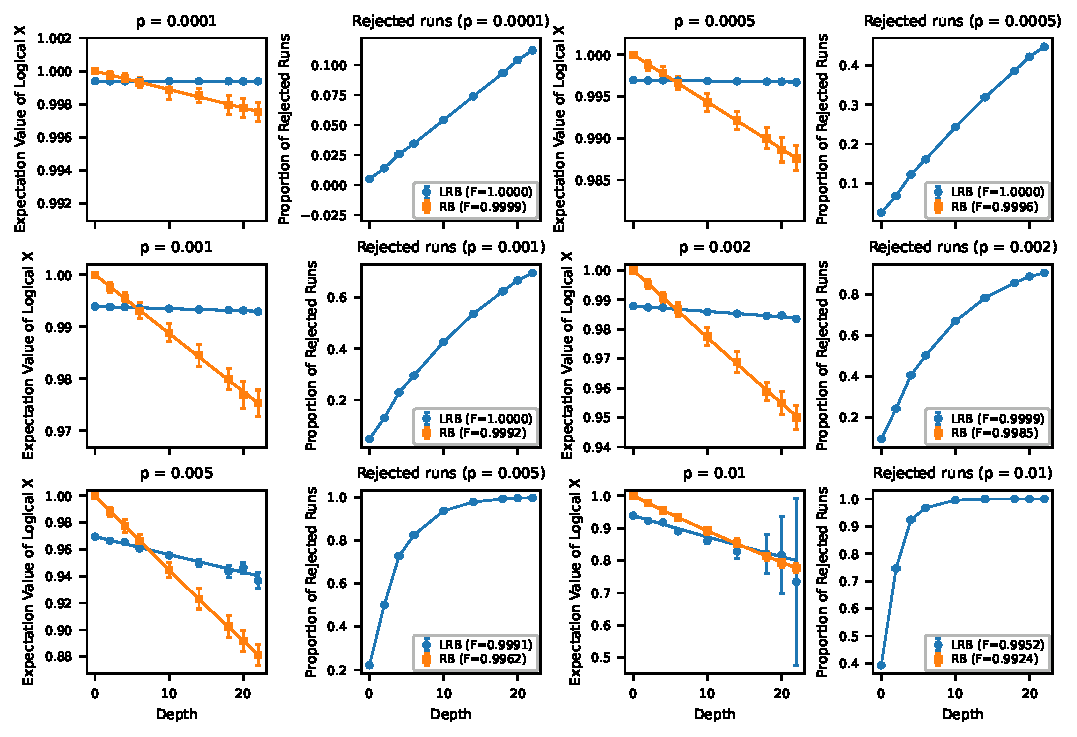
\includegraphics[width=0.78\textwidth]{figures/sdim140/si1000-1anc-unif-4-fit.pdf}
  \caption{Uniform-interval postselection with $k = 4$, one-ancilla layout, SI1000 ($\chi^2 = 9.1$ over nine depths at $p = 5\times10^{-3}$). At $p = 5\times10^{-3}$ the fitted error per unit depth is $9.3\times10^{-4}$, and at $p = 10^{-2}$ it is $4.8\times10^{-3}$, against $7.6\times10^{-3}$ for RB.}
  \label{fig:unif4_si1000_1anc}
\end{figure}

\begin{figure}[H]
  \centering
  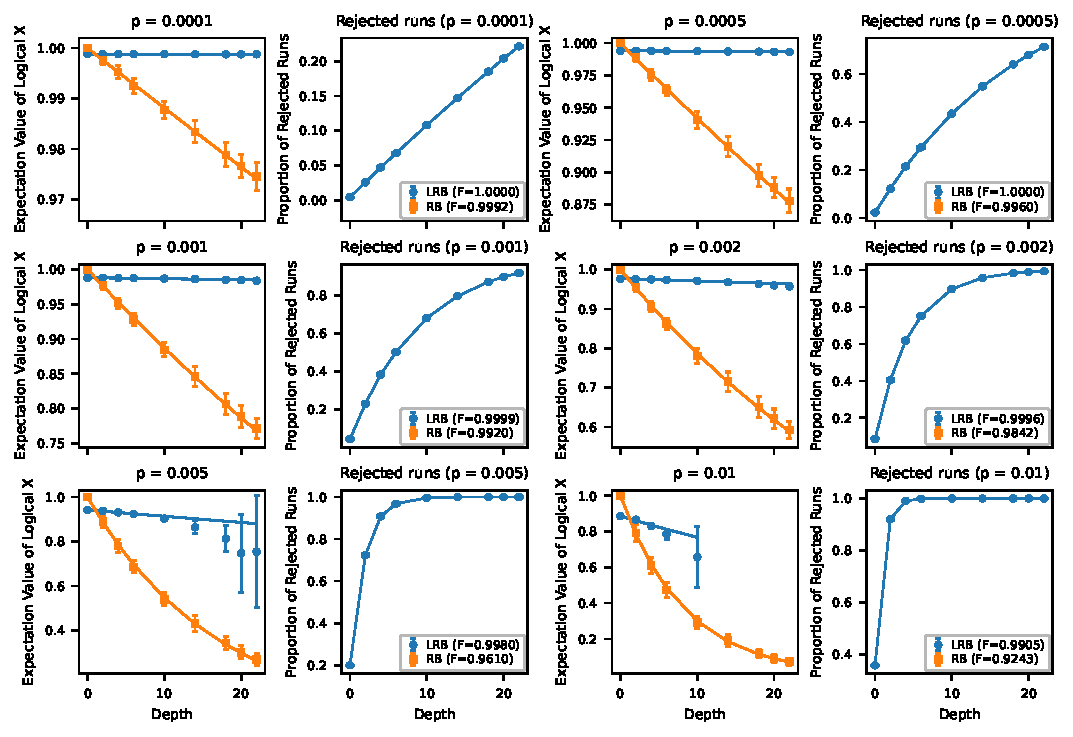
\includegraphics[width=0.78\textwidth]{figures/sdim140/sd6-1anc-unif-2-fit.pdf}
  \caption{Uniform-interval postselection with $k = 2$, one-ancilla layout, SD6, with RB under SD6 ($\chi^2 = 7.5$ over nine depths at $p = 5\times10^{-3}$). At $p = 10^{-2}$ the LRB-D fit uses five depths and gives an error per unit depth of $9.5\times10^{-3}$, against $7.6\times10^{-2}$ for RB.}
  \label{fig:unif2_sd6_1anc}
\end{figure}

\begin{figure}[H]
  \centering
  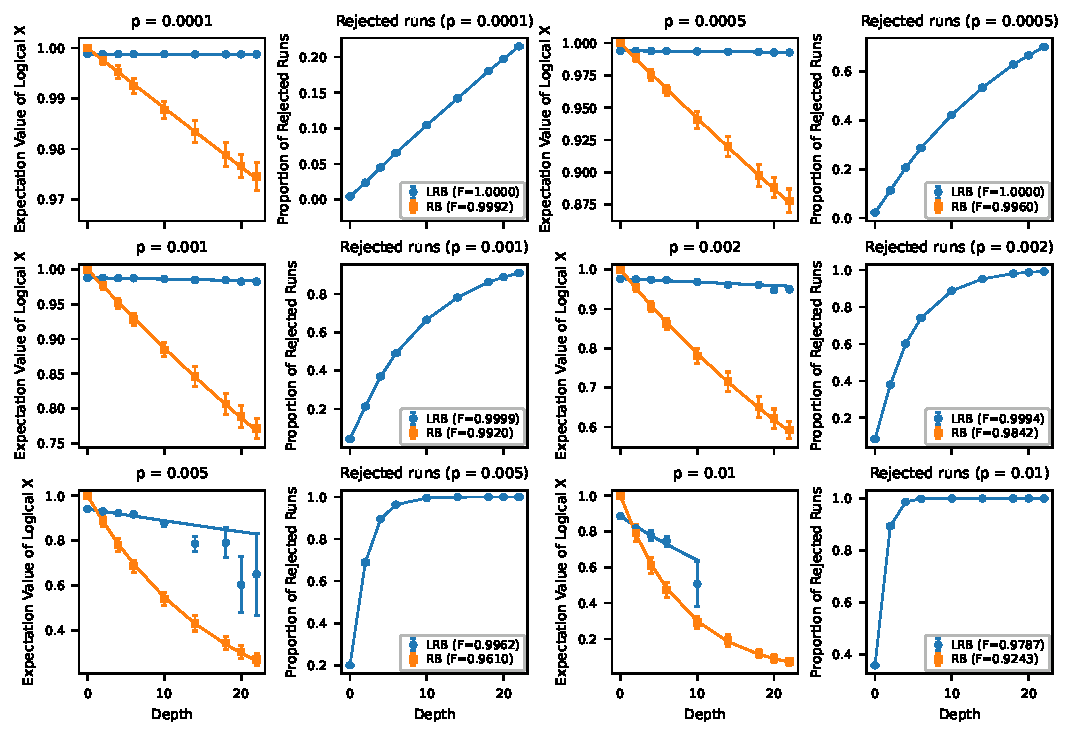
\includegraphics[width=0.78\textwidth]{figures/sdim140/sd6-1anc-unif-3-fit.pdf}
  \caption{Uniform-interval postselection with $k = 3$, one-ancilla layout, SD6 ($\chi^2 = 14.8$ over nine depths at $p = 5\times10^{-3}$). At $p = 10^{-2}$ the LRB-D fit uses five depths and gives an error per unit depth of $2.1\times10^{-2}$.}
  \label{fig:unif3_sd6_1anc}
\end{figure}

\begin{figure}[H]
  \centering
  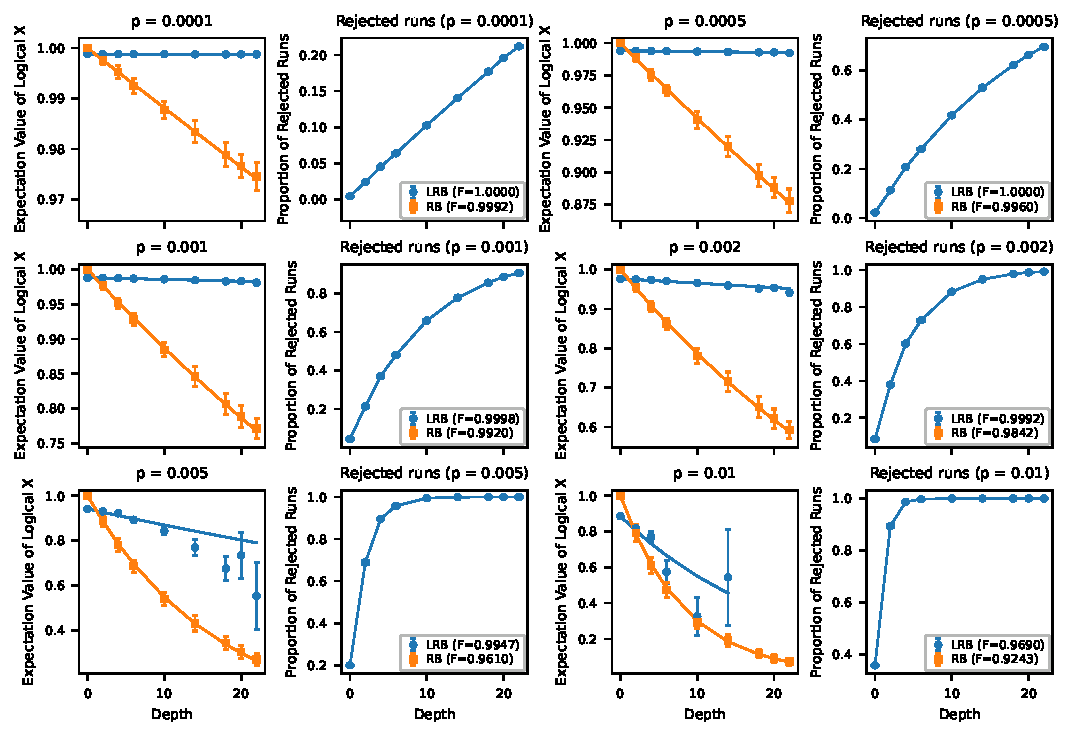
\includegraphics[width=0.78\textwidth]{figures/sdim140/sd6-1anc-unif-4-fit.pdf}
  \caption{Uniform-interval postselection with $k = 4$, one-ancilla layout, SD6 ($\chi^2 = 24.8$ over nine depths at $p = 5\times10^{-3}$). At $p = 10^{-2}$ the LRB-D fit uses six depths and gives an error per unit depth of $3.1\times10^{-2}$. Points that rest on a few accepted shots per sequence scatter upward (\autoref{sub:interval_results}).}
  \label{fig:unif4_sd6_1anc}
\end{figure}

\subsection{Two-Ancilla Layout}
% Rejected fractions, accepted <X> and fitted errors: paper-rework/facts/raw_per_depth.csv and fits_all_k.csv (conv-si1000, conv-sd6); depth counts and bracketing points of the threshold grids: paper-rework/scratch/writer-conv/analysis.py (sections A, A2, A3)

\begin{figure}[H]
  \centering
  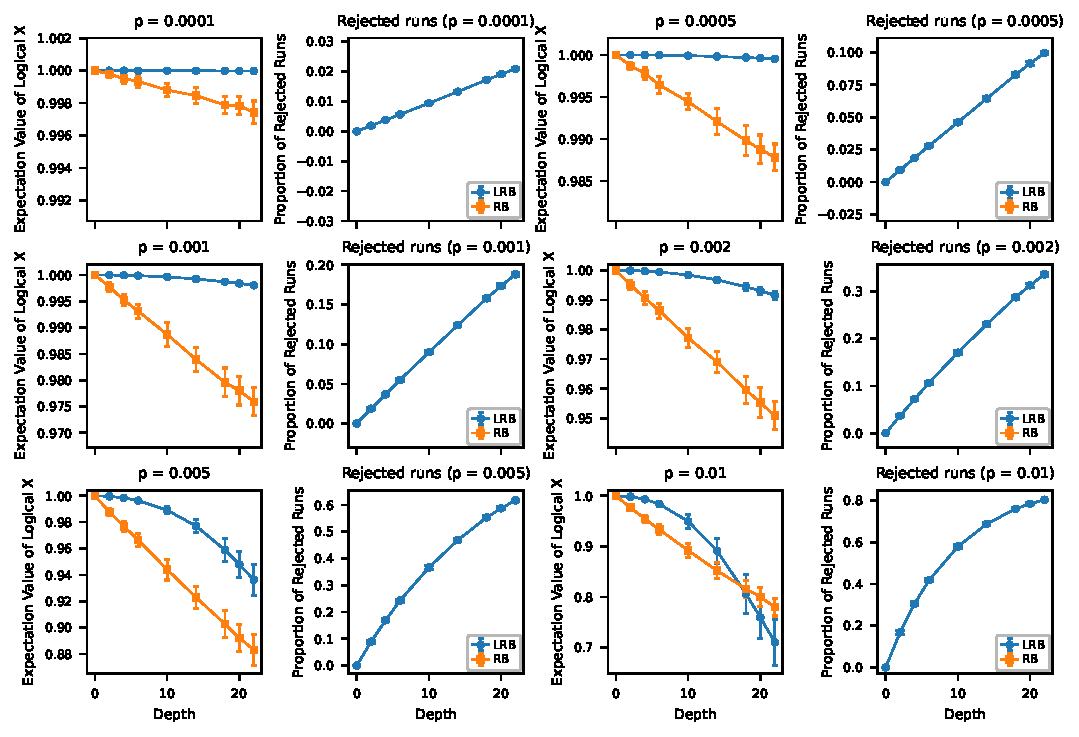
\includegraphics[width=0.78\textwidth]{figures/sdim140/si1000-conv-const-0-nofit.pdf}
  \caption{Terminal postselection (const-0), two-ancilla layout, SI1000. Without check rounds the two layouts run the same data circuits, and the ancillas only idle, so the traces agree with \autoref{fig:const0_si1000_1anc} up to the independent draw of the 30 sequences. At $p = 5\times10^{-3}$ and $m = 22$, for example, $\langle \bar{X} \rangle = 0.936$ and the rejected fraction is $0.617$, against $0.935$ and $0.622$ for one ancilla.}
  \label{fig:const0_si1000_2anc}
\end{figure}

\begin{figure}[H]
  \centering
  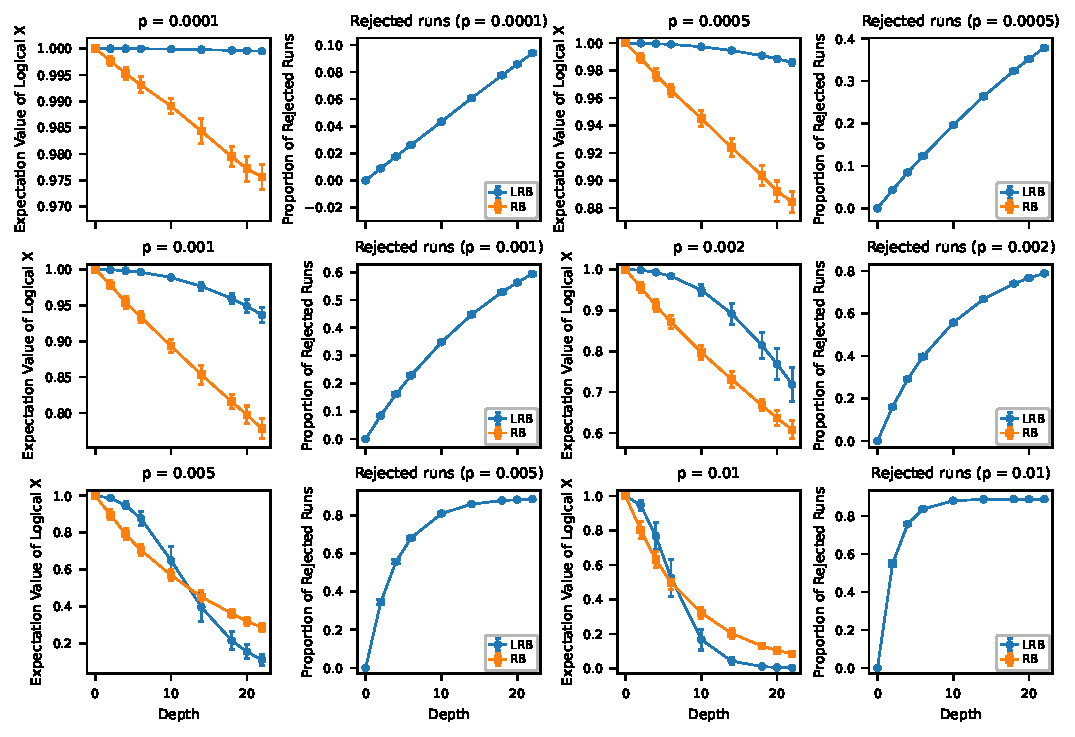
\includegraphics[width=0.78\textwidth]{figures/sdim140/sd6-conv-const-0-nofit.pdf}
  \caption{Terminal postselection (const-0), two-ancilla layout, SD6. As in \autoref{fig:const0_sd6_1anc}, the rejected fraction approaches $8/9$ (0.8889 at $p = 10^{-2}$ and $m = 22$).}
  \label{fig:const0_sd6_2anc}
\end{figure}

\begin{figure}[H]
  \centering
  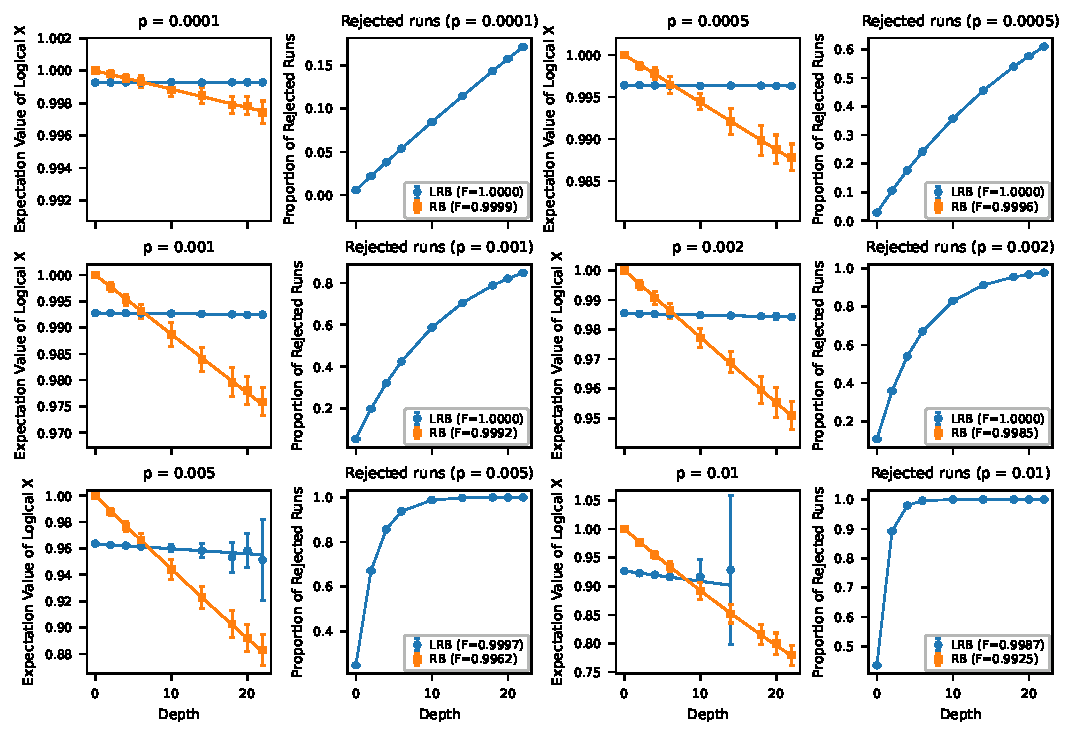
\includegraphics[width=0.78\textwidth]{figures/sdim140/si1000-conv-unif-1-fit.pdf}
  \caption{Uniform-interval postselection with $k = 1$, two-ancilla layout, SI1000. At $p = 5\times10^{-3}$ the rejected fraction at $m = 0$ is 25\% (22\% with one ancilla), the accepted $\langle \bar{X} \rangle$ at $m = 0$ is $0.964$ ($0.970$), and the fitted error per unit depth is $2.6\times10^{-4}$ ($2.3\times10^{-4}$), from a fit over nine depths.}
  \label{fig:unif1_si1000_2anc}
\end{figure}

\begin{figure}[H]
  \centering
  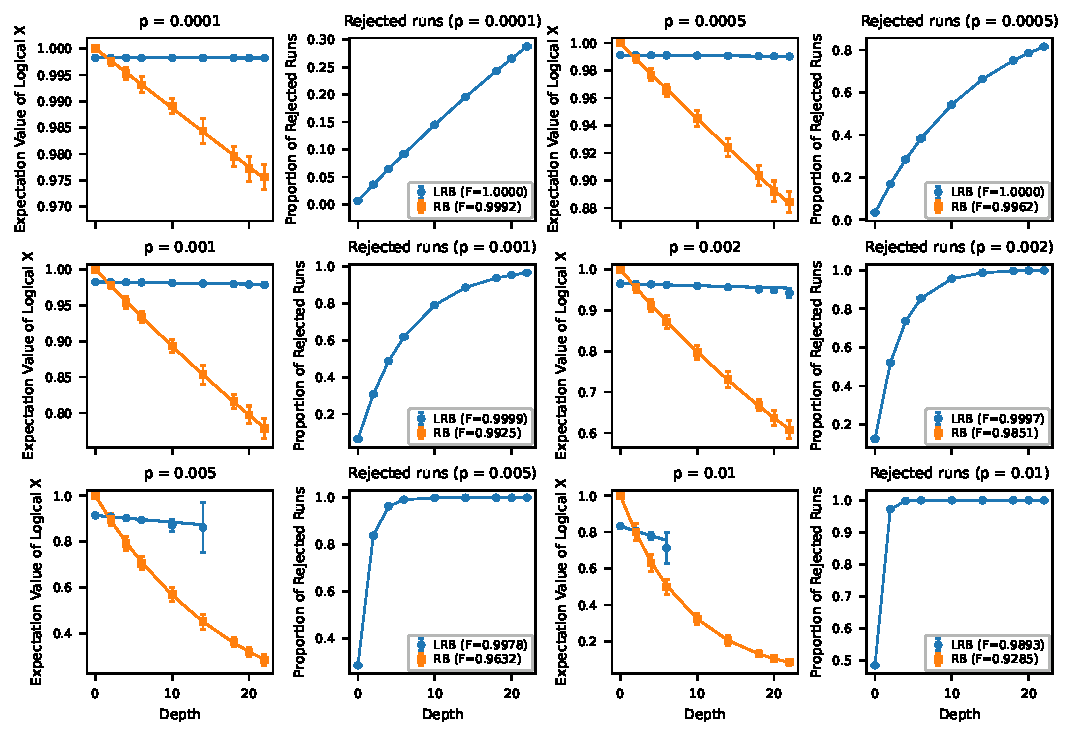
\includegraphics[width=0.78\textwidth]{figures/sdim140/sd6-conv-unif-1-fit.pdf}
  \caption{Uniform-interval postselection with $k = 1$, two-ancilla layout, SD6. At $p = 5\times10^{-3}$ the rejected fraction at $m = 0$ is 28\% (20\% with one ancilla), the accepted $\langle \bar{X} \rangle$ at $m = 0$ is $0.914$ ($0.941$), and the fitted error per unit depth is $2.2\times10^{-3}$ ($1.4\times10^{-3}$), from a fit over six depths.}
  \label{fig:unif1_sd6_2anc}
\end{figure}

\begin{figure}[H]
  \centering
  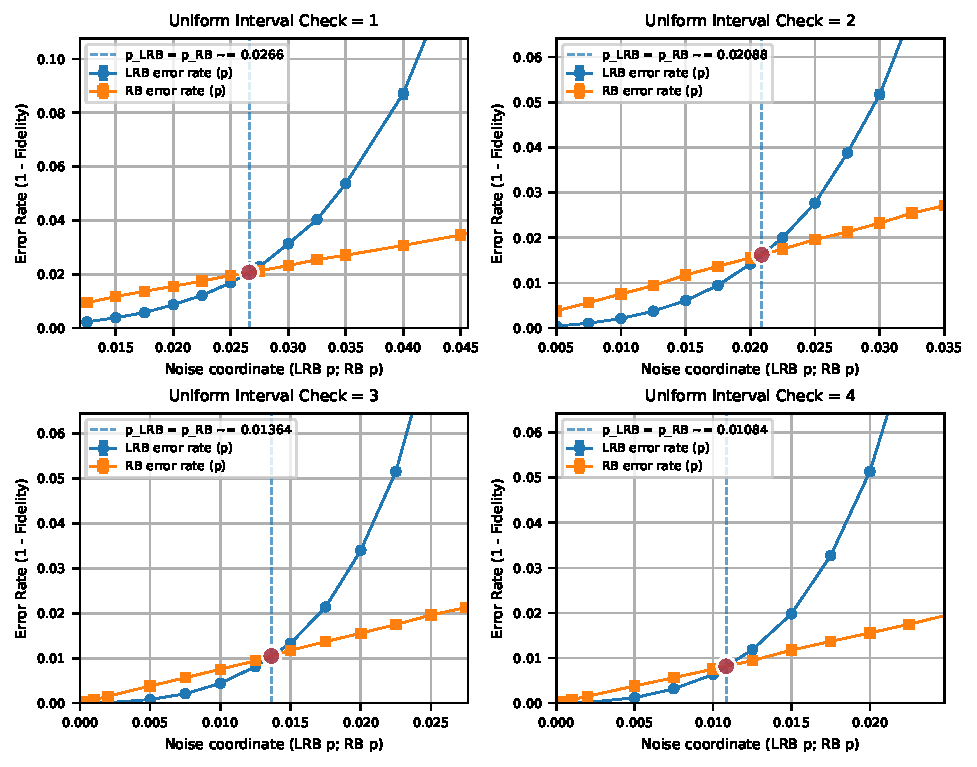
\includegraphics[width=0.85\textwidth]{figures/sdim140/si1000-conv-threshold-grid.pdf}
  \caption{Pseudo-threshold construction, two-ancilla layout, SI1000, with curves as in \autoref{fig:threshold_grid_si1000_1anc}. Points at $p < 0.015$ come from the production run, and points at $p \ge 0.015$ from the high-$p$ extension, fitted for $k = 1$ over four to six of its depths and for $k \ge 2$ over three or four of its even depths $0, 2, 4$ and $6$ (\autoref{sub:results_setup}). The markers are genuine crossings at $p^\star(k) = 0.0266$, $0.0209$, $0.0136$ and $0.0108$ for $k = 1$ to $4$. The $k = 1$ crossing lies between the extension points $0.025$ and $0.0275$, the $k = 2$ crossing between the extension points $0.02$ and $0.0225$, the $k = 3$ crossing between the production point $0.0125$ and the extension point $0.015$, and the $k = 4$ crossing between the production points $0.01$ and $0.0125$. The fits that bracket $p^\star(1)$ use six and five depths ($m \le 6$ and $m \le 4$), those that bracket $p^\star(2)$ use four, those that bracket $p^\star(3)$ use six ($m \le 14$) and four, and those that bracket $p^\star(4)$ use eight and six.}
  \label{fig:threshold_grid_si1000_2anc}
\end{figure}

\begin{figure}[H]
  \centering
  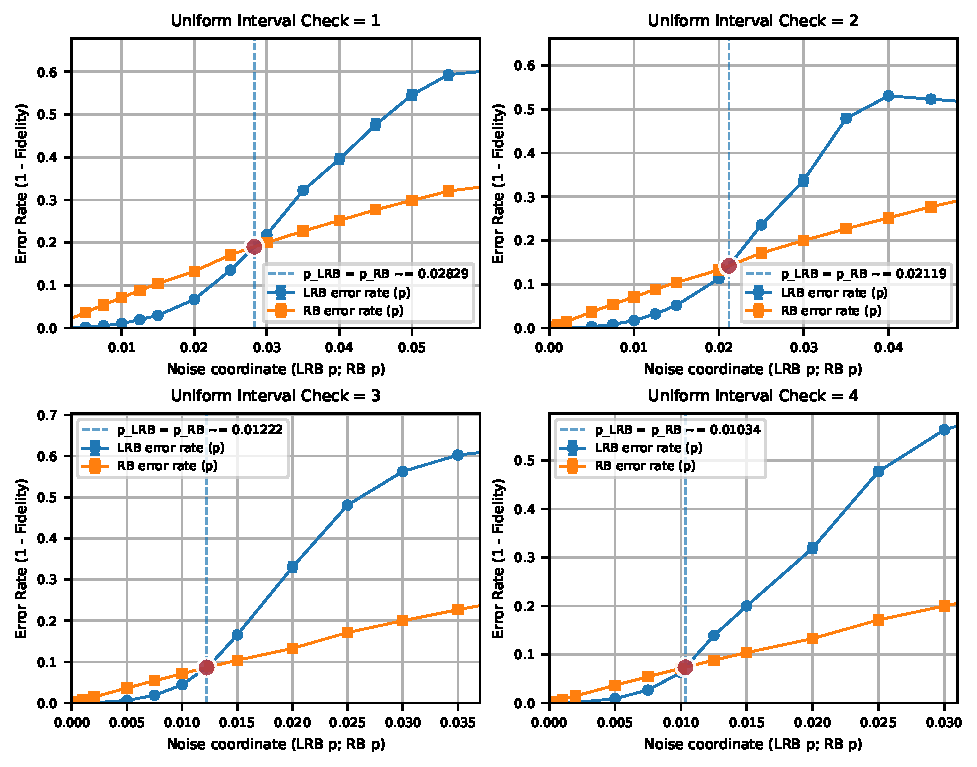
\includegraphics[width=0.85\textwidth]{figures/sdim140/sd6-conv-threshold-grid.pdf}
  \caption{Pseudo-threshold construction, two-ancilla layout, SD6, with curves as in \autoref{fig:threshold_grid_sd6_1anc}. Points at $p < 0.025$ come from the production run, and points at $p \ge 0.025$ from the high-$p$ extension. There the $k = 1$ fits use those extension depths at which every sequence keeps at least one shot, three to five depths with $m \le 4$, and the $k \ge 2$ fits use three or four of the even depths $0, 2, 4$ and $6$ (\autoref{sub:results_setup}). The markers are genuine crossings at $p^\star(k) = 0.0283$, $0.0212$, $0.0122$ and $0.0103$ for $k = 1$ to $4$. The $k = 1$ crossing lies between the extension points $0.025$ and $0.03$, the $k = 2$ crossing between the production point $0.02$ and the extension point $0.025$, and the $k = 3$ and $4$ crossings between the production points $0.01$ and $0.0125$. In the $k = 2$ panel the fitted LRB-D error falls slightly from $p = 0.04$ to $0.045$ ($0.531$ to $0.523$), with three depths at both points.}
  \label{fig:threshold_grid_sd6_2anc}
\end{figure}
